Die Abbildungen \ref{fig:Grafana_Gain0}-\ref{fig:Grafana_Gain3} zeigen die gleiche Messung eines Wolkenfreien Dezembertags am 12.12.2020 in Berlin mit unterschiedlichen verstärkungsfaktoren der Integrationswert ist auf 255 gesetzt.
Es ist zu erkennen, dass die Auflösung der Y-Achse mit zunehmender Verstärkung steigt. Aus Abbildung 3 ist jedoch ersichtlich, dass der maximale Messwert von 65.000 mit einem hohen Verstärkungsfaktor erreicht werden kann und die Daten so ihre Aussagekraft verlieren (clipping).

Abbildung \ref{fig:Grafana_AutoGain} zeigt die gleiche Messung im AutoGain-Modus, hier werden die Messungen mit den verschiedenen Verstärkungsfaktoren zusammengefasst und in einem Plot mit maximaler Auflösung, aber ohne Clipping dargestellt.
Durch auswahl der Integrationszeit und der Durchlässigkeit der Streuscheibe muss sichergestellt werden, dass bei Gain 0 kein Clipping auftritt.

Die Ausgabe-Daten der Messung sind nicht kalibriert.
Außerdem haben sie keine Einheit bei festem Gain liegen sie zwischen 0 und 65000.
Im Autogain-Modus liegen sie zwischen 0 und 4160000.
Um die Daten nutzbar zu machen, müssen sie mit Hilfe eines anderen Messgerätes auf allgemein verständliche Candela-Werte kalibriert werden.

\begin{figure}[H]
\centering
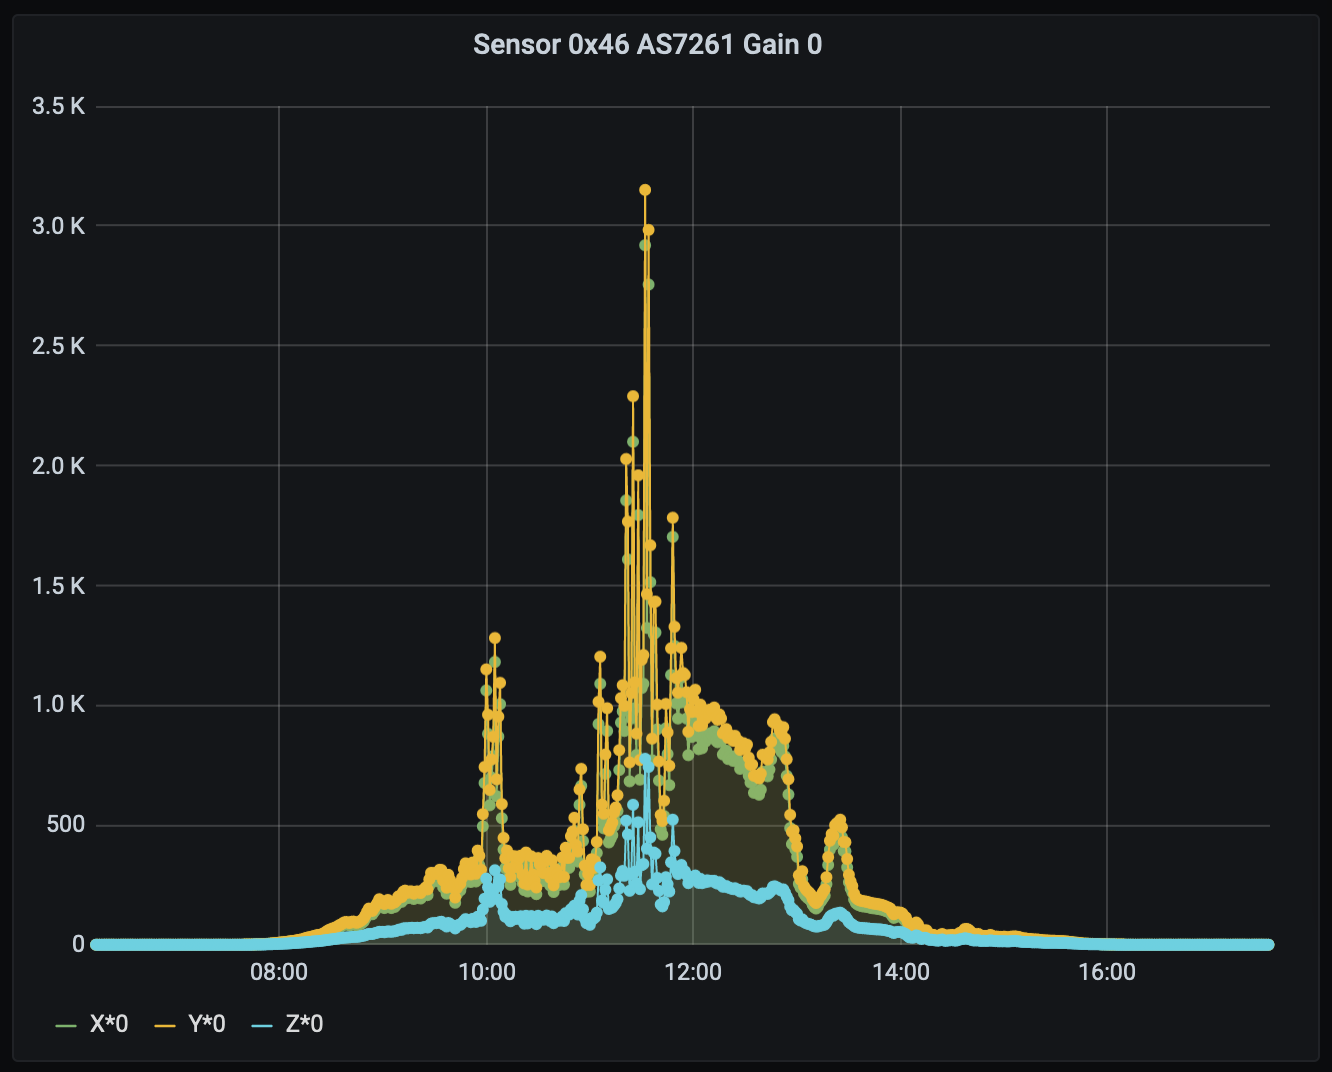
\includegraphics[width=0.6\textwidth]{img/Grafana-Gain0}
\caption{Gain 0 (1x)}
\label{fig:Grafana_Gain0}
\end{figure}

\begin{figure}[H]
\centering
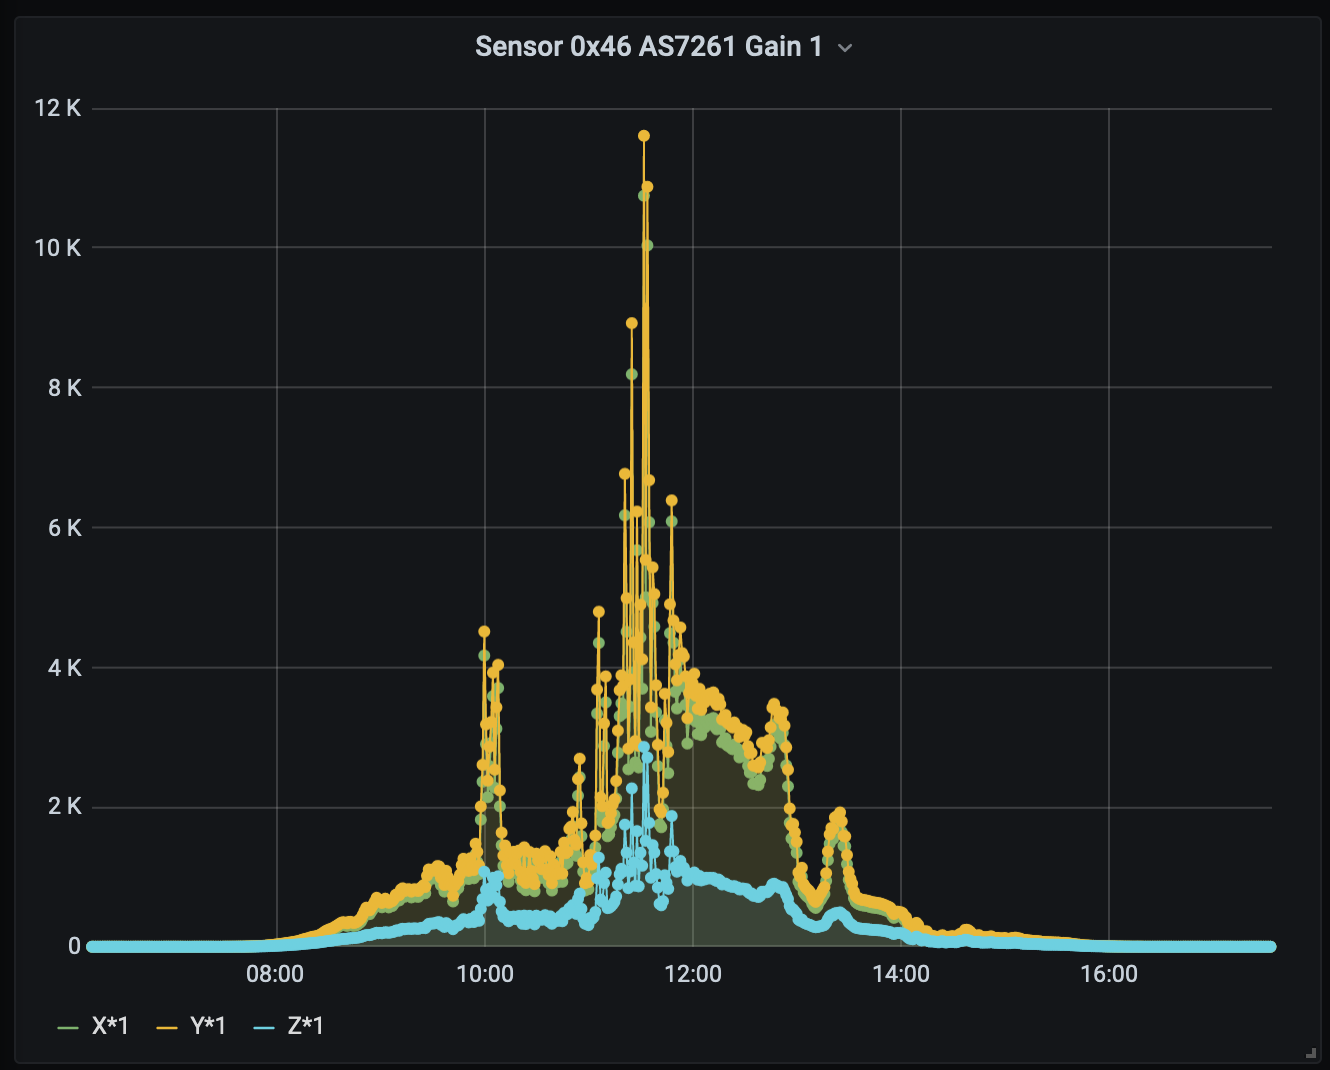
\includegraphics[width=0.6\textwidth]{img/Grafana-Gain1}
\caption{Gain 1 (3,7x)}
\label{fig:Grafana_Gain1}
\end{figure}

\begin{figure}[H]
\centering
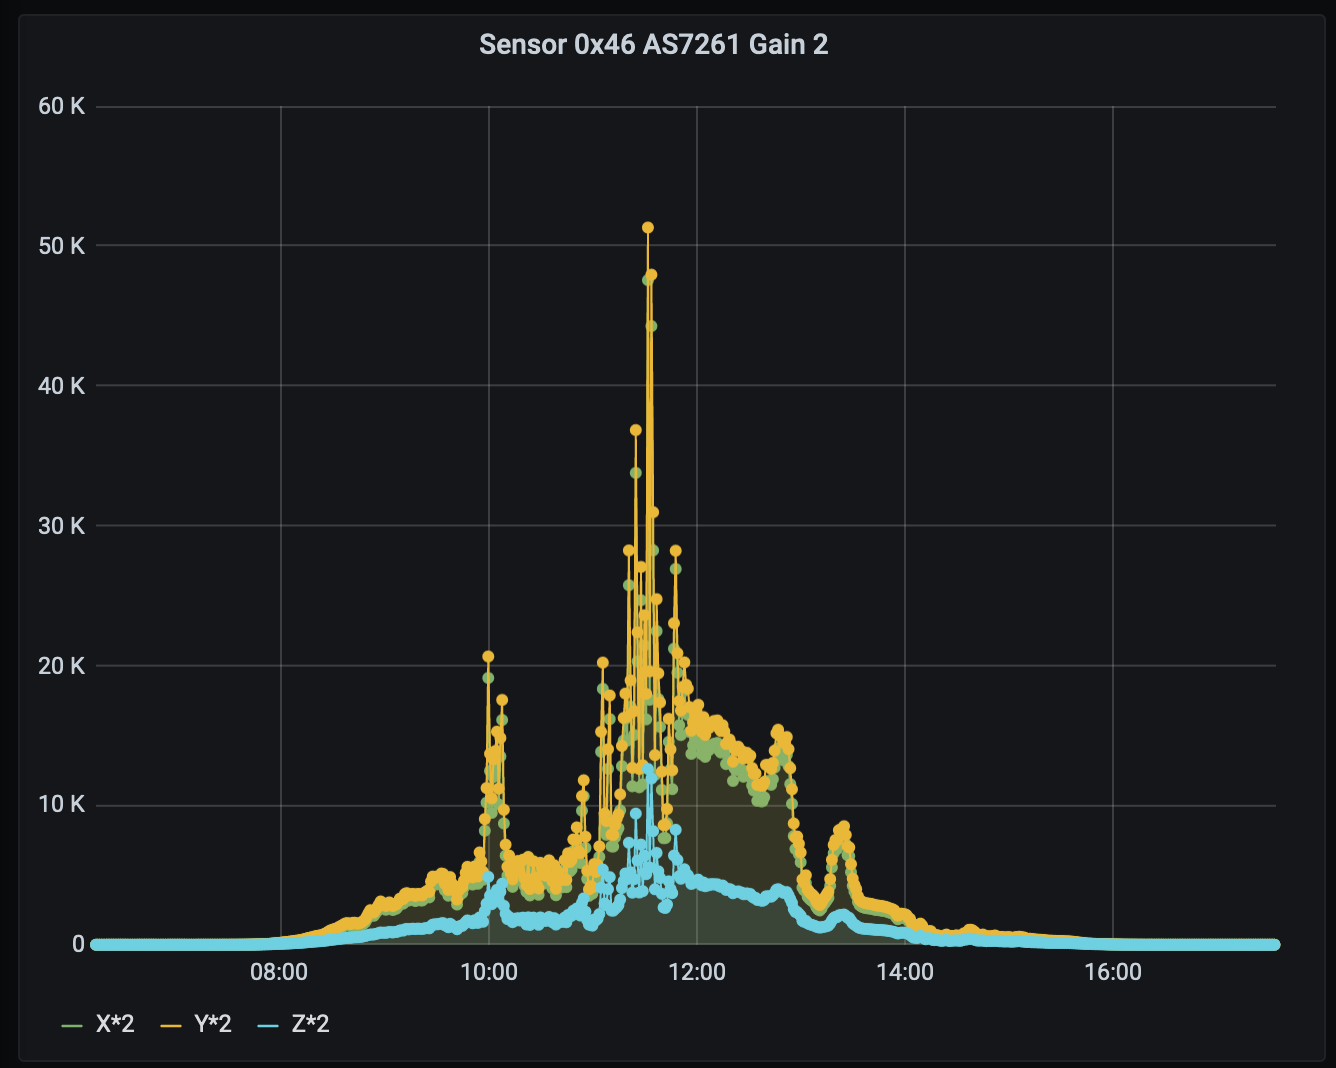
\includegraphics[width=0.6\textwidth]{img/Grafana-Gain2}
\caption{Gain 2 (16x)}
\label{fig:Grafana_Gain2}
\end{figure}

\begin{figure}[H]
\centering
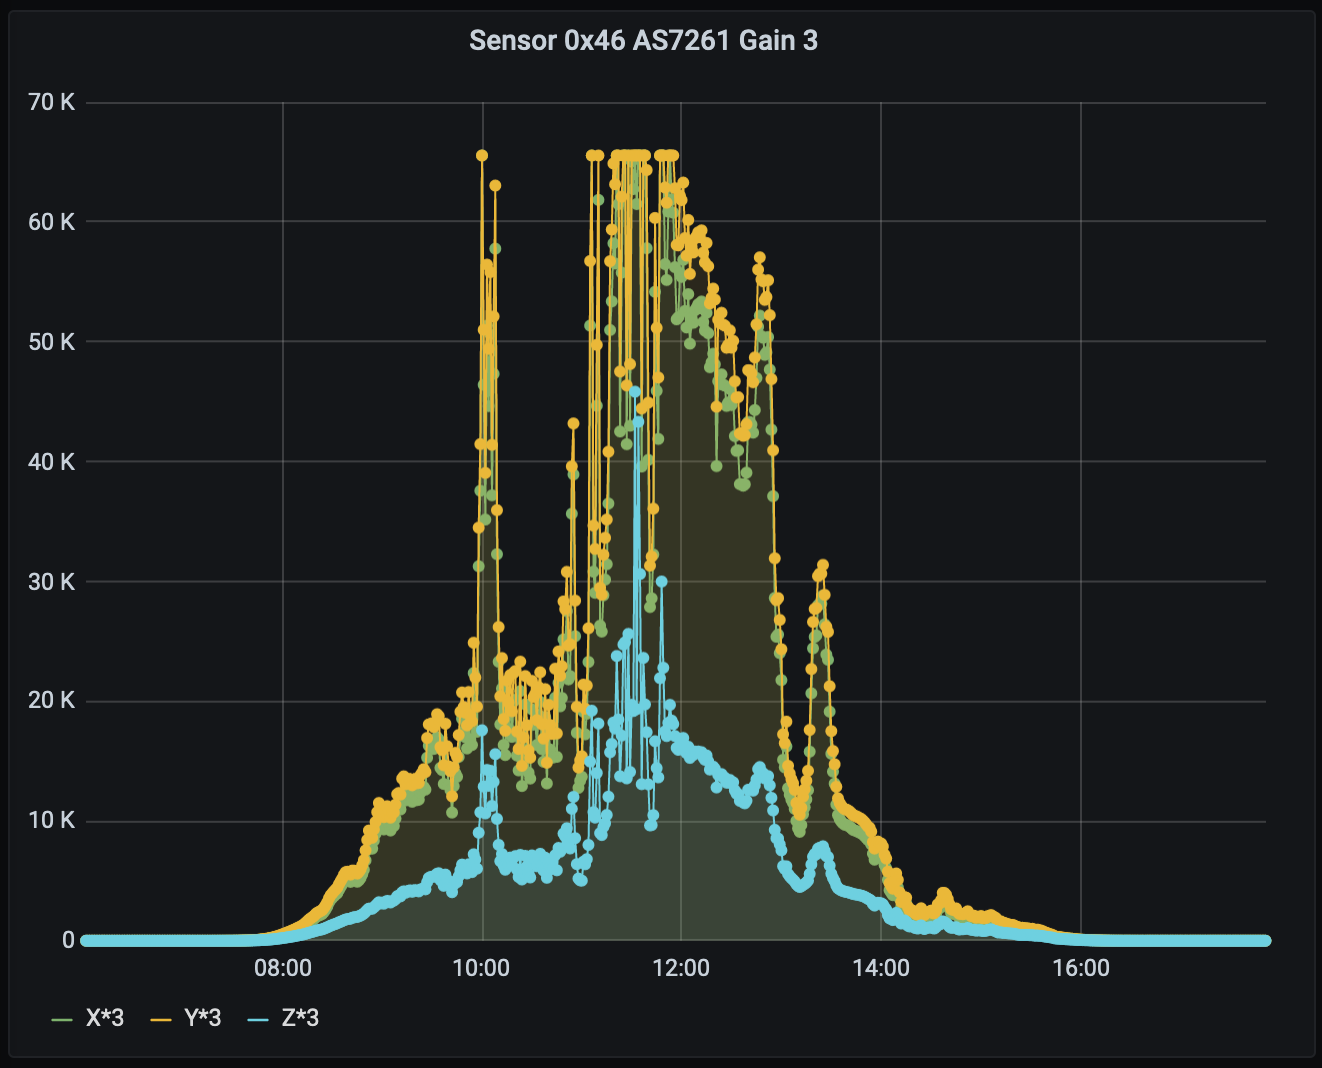
\includegraphics[width=0.6\textwidth]{img/Grafana-Gain3}
\caption{Gain 3 (64x)}
\label{fig:Grafana_Gain3}
\end{figure}

\begin{figure}[H]
\centering
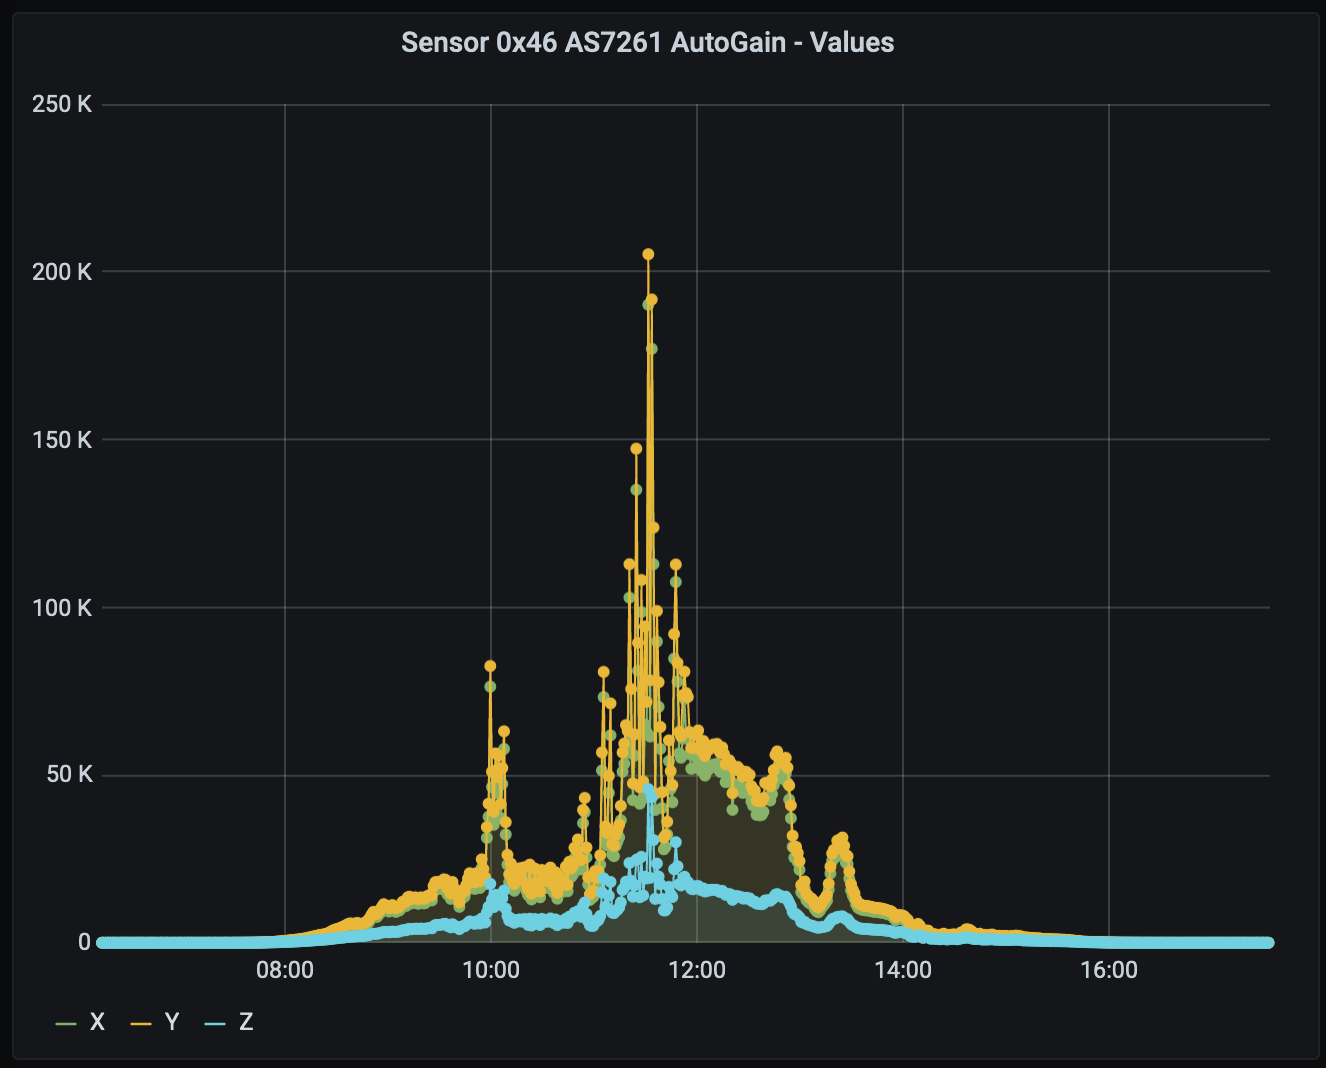
\includegraphics[width=0.6\textwidth]{img/Grafana-AutoGain}
\caption{AutoGain}
\label{fig:Grafana_AutoGain}
\end{figure}